\documentclass{article}

\usepackage{amsmath}
\usepackage{graphicx}
\usepackage{subcaption}
\usepackage{bigfoot}
\usepackage{hyperref}

\title{Controlling a Servo Motor with PWM}
\date{19 September 2018}
\author{
	ECE 388
	\\
	\\
	Team 4:
	\\
	Jacob Aubertine (jacobaubertine)
	\\
	Mathieu Bolduc-Clayton (mclayton820)
	\\
	Sal Fernandes (sfernandes2)
	\\
	\\
	(GitHub usernames in parentheses)
}

\begin{document}
	\pagenumbering{gobble}
	\maketitle
	\newpage
	\pagenumbering{arabic}

	\section{SG90 Servo Motor}
	The goal of the first lab meeting was to control a servo motor using pulse-width modulation (PWM). Since the group was not familiar with the specific motor given (SG90), its datasheet was found online. The servo could only rotate 180 degrees, and the duty cycle determined what position it would be in. The recommended period for the PWM signal was 20 ms (50 Hz), with a duty cycle of between 5\% and 10\%. A 5\% duty cycle (1 ms) rotated the motor to -90 degrees, while a 10\% duty cycle rotated the motor to +90 degrees. This information is shown in Table \ref{tab:table1}. There were three wires leading from the motor: orange was PWM, red was VCC, and brown was ground. This information was found in the datasheet online\footnote{\href{http://www.ee.ic.ac.uk/pcheung/teaching/DE1_EE/stores/sg90_datasheet.pdf}{Imperial College London Engineering website on a professor's class page}}.

	% table
	\begin{table}[h!]
  		\begin{center}
    			\caption{Pulse widths and corresponding positions.}
    			\label{tab:table1}
    			\begin{tabular}{r|r}
      				\textbf{Pulse width} & \textbf{Position (deg)} \\
				\hline
      				1 ms& -90 deg\\
      				1.25 ms & -45 deg\\
      				1.5 ms & 0 deg\\
      				1.75 ms & 45 deg\\
				2 ms& 90 deg\\
   			 \end{tabular}
  		\end{center}
	\end{table}

	\section{Function Generator Setup}
	To create the PWM signal, the function generator was used. The pulse setting was used, with a 50 Hz frequency and 5 Vpp amplitude as defined in the datasheet. To get the signal to go from 0 to 5 V instead of -2.5 V to 2.5 V, a 2.5 V\textsubscript{DC} offset was used. The edge width was left unchanged at 50 ns. The oscilloscope displaying a 1.5 ms pulse with a 20.0 ms period is shown in Figure \ref{fig:oscilloscope}.

	% figure
	\begin{figure}[h!]
		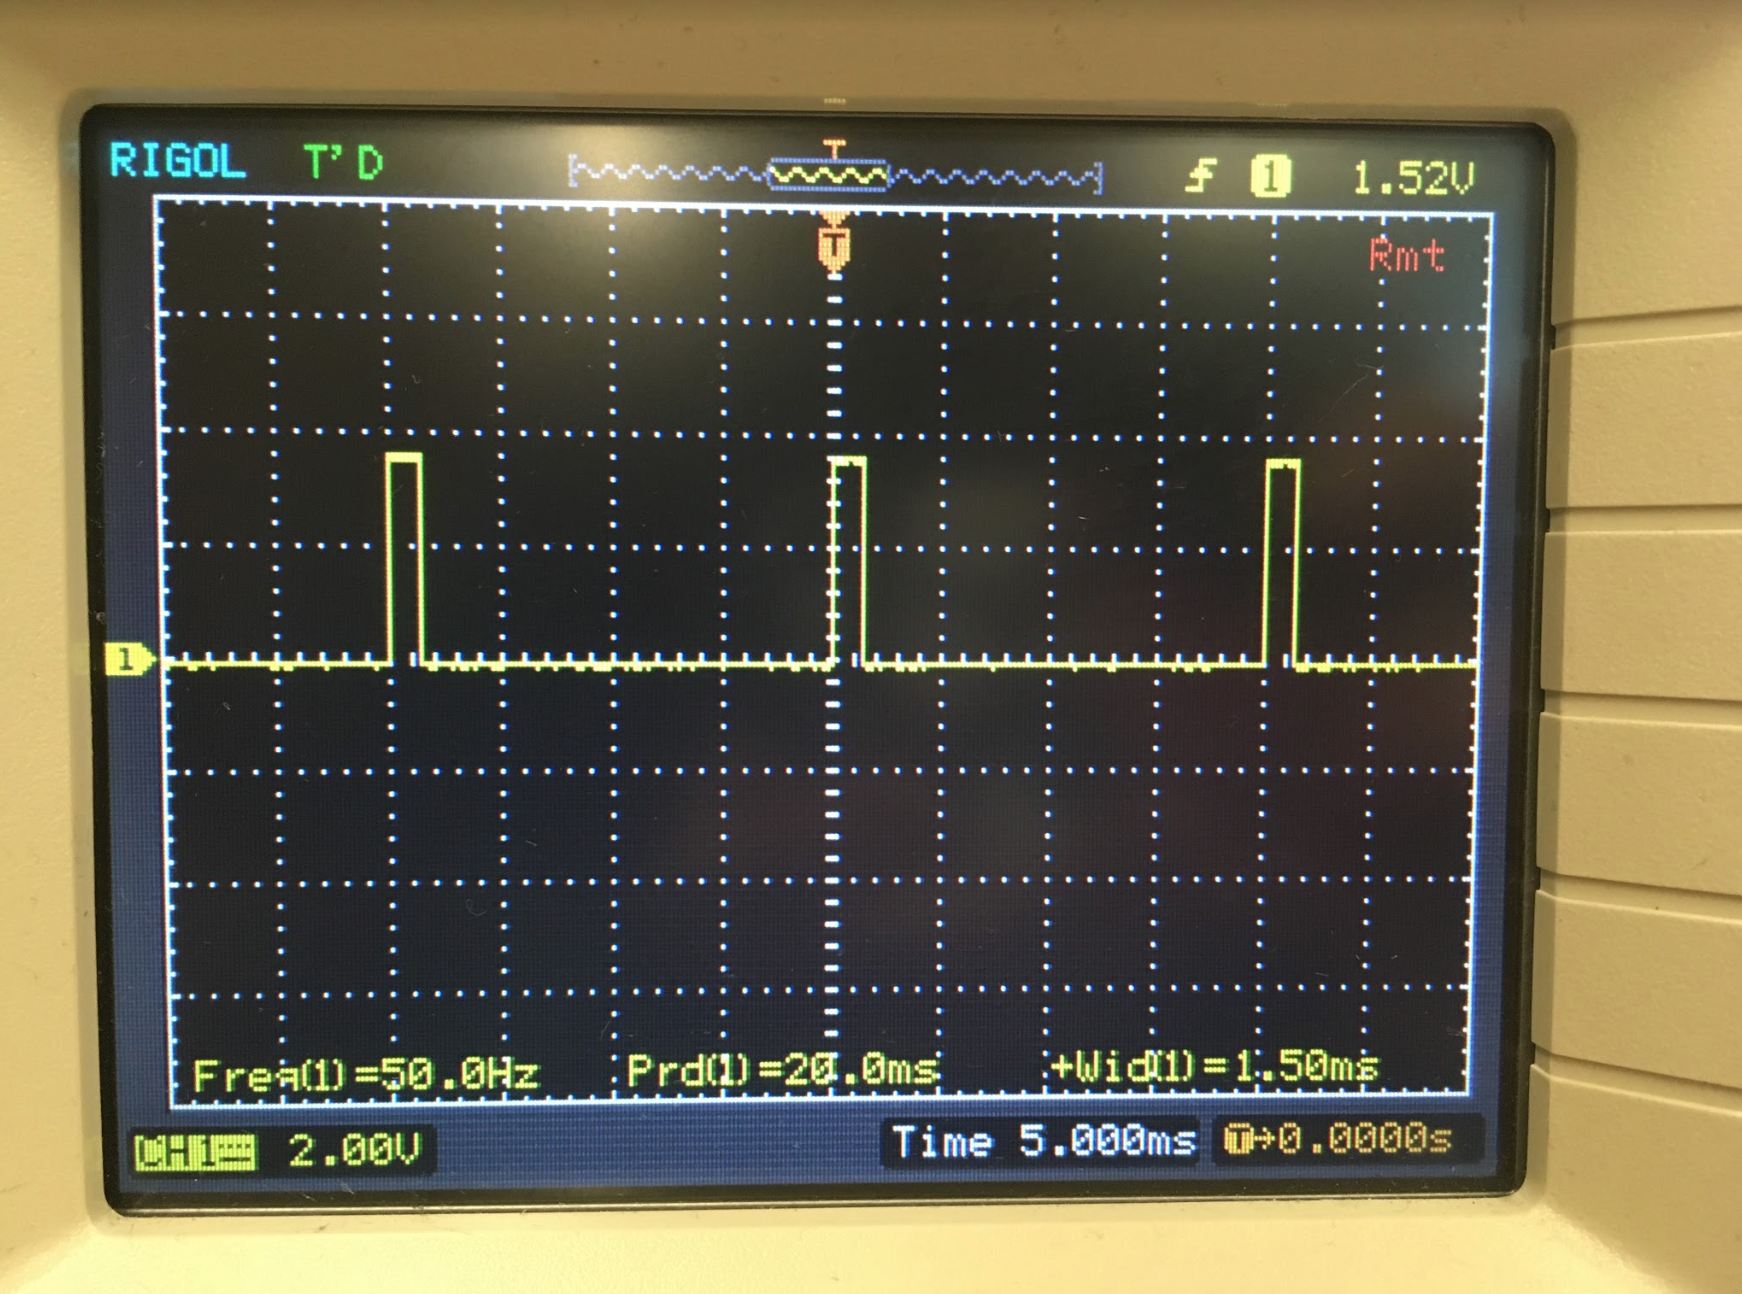
\includegraphics[width=\linewidth]{oscilloscope.png}
		\caption{Oscilloscope readings when connected to function generator.}
		\label{fig:oscilloscope}
	\end{figure}

\end{document}